\documentclass[12pt]{report}
\usepackage[catalan]{babel}
%\usepackage[latin1]{inputenc}   % Permet usar tots els accents i car�ters llatins de forma directa.
\usepackage[utf8]{inputenc}  
\usepackage{enumerate}
\usepackage{amsfonts, amscd, amsmath, amssymb}
\usepackage[pdftex]{graphicx}

\setlength{\textwidth}{16cm}
\setlength{\textheight}{24.5cm}
\setlength{\oddsidemargin}{-0.3cm}
\setlength{\evensidemargin}{0.25cm} \addtolength{\headheight}{\baselineskip}
\addtolength{\topmargin}{-3cm}

\newcommand\Z{\mathbb{Z}}
\newcommand\R{\mathbb{R}}
\newcommand\N{\mathbb{N}}
\newcommand\Q{\mathbb{Q}}
\newcommand\K{\Bbbk}
\newcommand\C{\mathbb{C}}

\newcounter{exctr}
\newenvironment{exemple}
{ \stepcounter{exctr} 
\hspace{0.2cm} 
\textit{Exemple  \arabic{exctr}: }
\it
\begin{quotation}
}{\end{quotation}}

\pagestyle{empty}

\begin{document}

\begin{center}
\textbf{\Large Càlcul II.\\ Control 1. Curs 2011-12}
\end{center}

\vskip 0.3cm
\noindent
\textbf{P1.} Associau cada una de les següents funcions a un gràfica i a un mapa de corbes de nivell. Justificau
la resposta. Calculau al menys una corba de nivell per a cada funció.
\begin{enumerate}[a)]
\item $f(x, y)=x^3-3xy^2$
\item $f(x, y)=sin\sqrt{x^2+y^2}$
\item $f(x, y)=\frac{1}{x^2+4y^2}$
\end{enumerate}


\begin{figure}[htbp]
\begin{center}
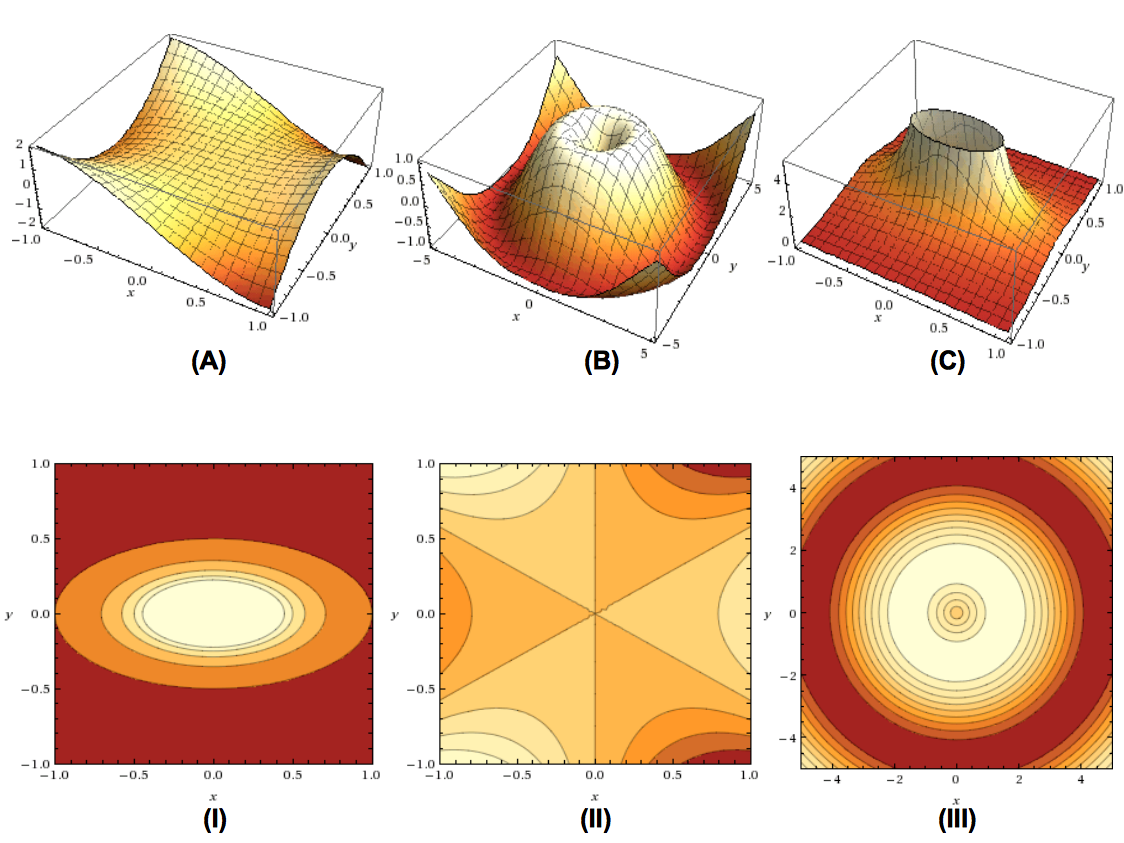
\includegraphics[width=12cm]{figura1.png}
\end{center}
\end{figure}

\vskip 0.3cm
\noindent
\textbf{P2.} Considerau el següent límit:
\[
\lim_{(x, y) \rightarrow (1, 4)} e^{\sqrt{x+2y}}
\]

\begin{enumerate}[a)]
\item calculau els límits iterats
\item calculau els límits segons les rectes que passen per $(1, 4)$
\item calculau el límit, si existeix
\item determinau si la funció és contínua en $(1, 4)$
\end{enumerate} 



\vskip 0.8cm
\noindent
\textbf{Formulari}

\begin{enumerate}
\item equació d'una circumferència de radi $r$ i centre $(a, b)$: $(x-a)^2+(y-b)^2=r^2$
\item equació d'una elipse centrada en $(0, 0)$: $\frac{x^2}{a^2}+\frac{y^2}{b^2}=1$
\item equació d'una hipèrbola centrada en $(0, 0)$: $\frac{x^2}{a^2}-\frac{y^2}{b^2}=1$
\end{enumerate}


\end{document}